\documentclass[a4paper,10pt]{article}
\usepackage{mystyle}
\usepackage[top=3cm, bottom=3cm, left=3cm, right=3cm]{geometry}
\def\labelitemi{---}

\begin{document}

\title{\texttt{PrefixCCFWC}: performance comparison}
\author{Victor Lecomte}
\maketitle

\begin{abstract}
For the PrefixCC problem, whose statement is described in the main technical report, we implemented several approaches with different complexities and pruning levels. In order to decide which ones to keep, we performed several benchmarks, which we present here with results, comments and conclusions.
\end{abstract}

\tableofcontents

\section{Approaches}

Four approaches were considered for the performance testing:
\begin{itemize}
    \item \emph{Multiple GCCFWCs}: our baseline, which consists in adding as many regular \texttt{GCCFWC} constraints as there are prefixes constrained.
    
    This approach is expected to be slow because of the redundancy of the reversible structures and simply the large number of constraints to be queued at each node.
    \item \emph{PrefixCC Segments}: the main approach, described in the accompanying technical report. First performs some deduction and filtering on the bounds and then prunes according to those but in an efficient non-redundant way, by working segment-by-segment instead of prefix-by-prefix.
    
    This approach is expected to stay quick even for a large number of variables.
    \item \emph{PrefixCC Fenwick}: another efficient approach, that makes the same types of deductions as the previous ones but also takes into account the current state of the variables. According to that, it keeps with a Fenwick tree the dynamic list of the best-known bounds for each prefix and prunes values every time the lower and upper bounds become equal in an interval. In that way it is, for each value, arc-consistent on the subset of bounds relative to the value.
    
    This approach is expected to have a better pruning.
    \item \emph{PrefixCC Embedded GCCFWCs}: same as the segments one except that once the bounds are deducted and filtered it keeps a separate count for each constraint which is a bit more redundant (but not as much as the baseline).
    
    This approach is expected to be quick for small numbers of variables.
\end{itemize}

\section{Tests performed}

Two kinds of tests were performed:
\begin{itemize}
    \item test cases where the lower bounds and upper bounds were very weak so that pruning matters only very little and raw propagation speed is shown;
    \item harder test cases where solutions are harder to find and backtracks take up most of the time, in order to isolate the solutions with the best pruning.
\end{itemize}

This section describes the methodology for generating those test cases. We will first touch the common aspects of the benchmarks (\ref{subsec:tests-common}) and then explain the differences between them (\ref{subsec:tests-weak} and \ref{subsec:tests-hard}).

\subsection{Common aspects}
\label{subsec:tests-common}
For every test, we picked a certain number of variables \texttt{nVariables}. We mostly used 50, 100 and 200 variables to make our tests. Each variable was given a random domain among three possible values.

We then added \texttt{nVariables} lower bounds and \texttt{nVariables} upper bounds by choosing a random prefix and a random value to constrain. The actual bounds depended on the benchmark. Given that there are three values, this makes for one bound for each value every three prefixes in average. Such a quantity of bounds was necessary to pick up with clarity the complexities of the approaches relative to the number of bounds.

After that we started a binary static search with the table of variables shuffled in the same way for every approach. The shuffling avoided stumbling upon a special case with a better complexity for some approaches. The search stopped after finding a set number of solutions.

For every test, the approaches were run in a random order to remove undesirable biases due to JVM warmup.

\subsection{Weak constraints}
\label{subsec:tests-weak}

In this benchmark, in order to measure the raw propagation speed of the approaches, we made the solutions very easy to find. To do that, we gave the bounds very conservative values.

We simply assigned the lower bounds to $1/7$ of the size of the prefix and the upper bounds to $6/7$ of the size of the prefix. Since there are only three values those bounds are nearly always respected and we could compare the approaches as they went through similar search trees.

\subsection{Harder cases}
\label{subsec:tests-hard}

In this benchmark, we wanted to give cases where finding solutions is more tricky so that the solutions with the best pruning have an advantage. But there still had to be some solutions so that we can time the approaches correctly.

To do that, we took a random solution with respect to the domains of the variables and we based the bounds on the effective occurrences of the values in that solution. We allowed lower bounds to vary randomly between $75\%$ and $100\%$ of the number of occurrences in the model solution, and upper bounds to vary randomly between $100\%$ and $125\%$ of the number of occurrences in the model solution. That way we had strong bounds but still at least one solution (and probably many more).

We also tried narrower intervals for the lower bounds and upper bounds but all solutions except the one with the best pruning ended up timing out, which was comforting but did not give interesting data.

Since the running time would get quite high for this type of problem with the solutions that performed little pruning, we chose to run them only for 50 variables, as the results were already enough to draw conclusions.

\section{Commented results}

We will now present the test results for the different approaches and draw general tendencies from them.

\subsection{Weak constraints tests}
\label{subsec:results-weak}

As mentioned before, the aim of the tests with weak constraints was to measure raw propagation speed. We first wanted to evaluate roughly how that speed evolved with the number of variables, so we performed quick tests to get a rough idea. Figure~\ref{fig:loglog-complexity} shows the total search time divided by the number of nodes for each approach, at 20, 50, 100 and 200 variables.

\begin{figure}
    \centering
    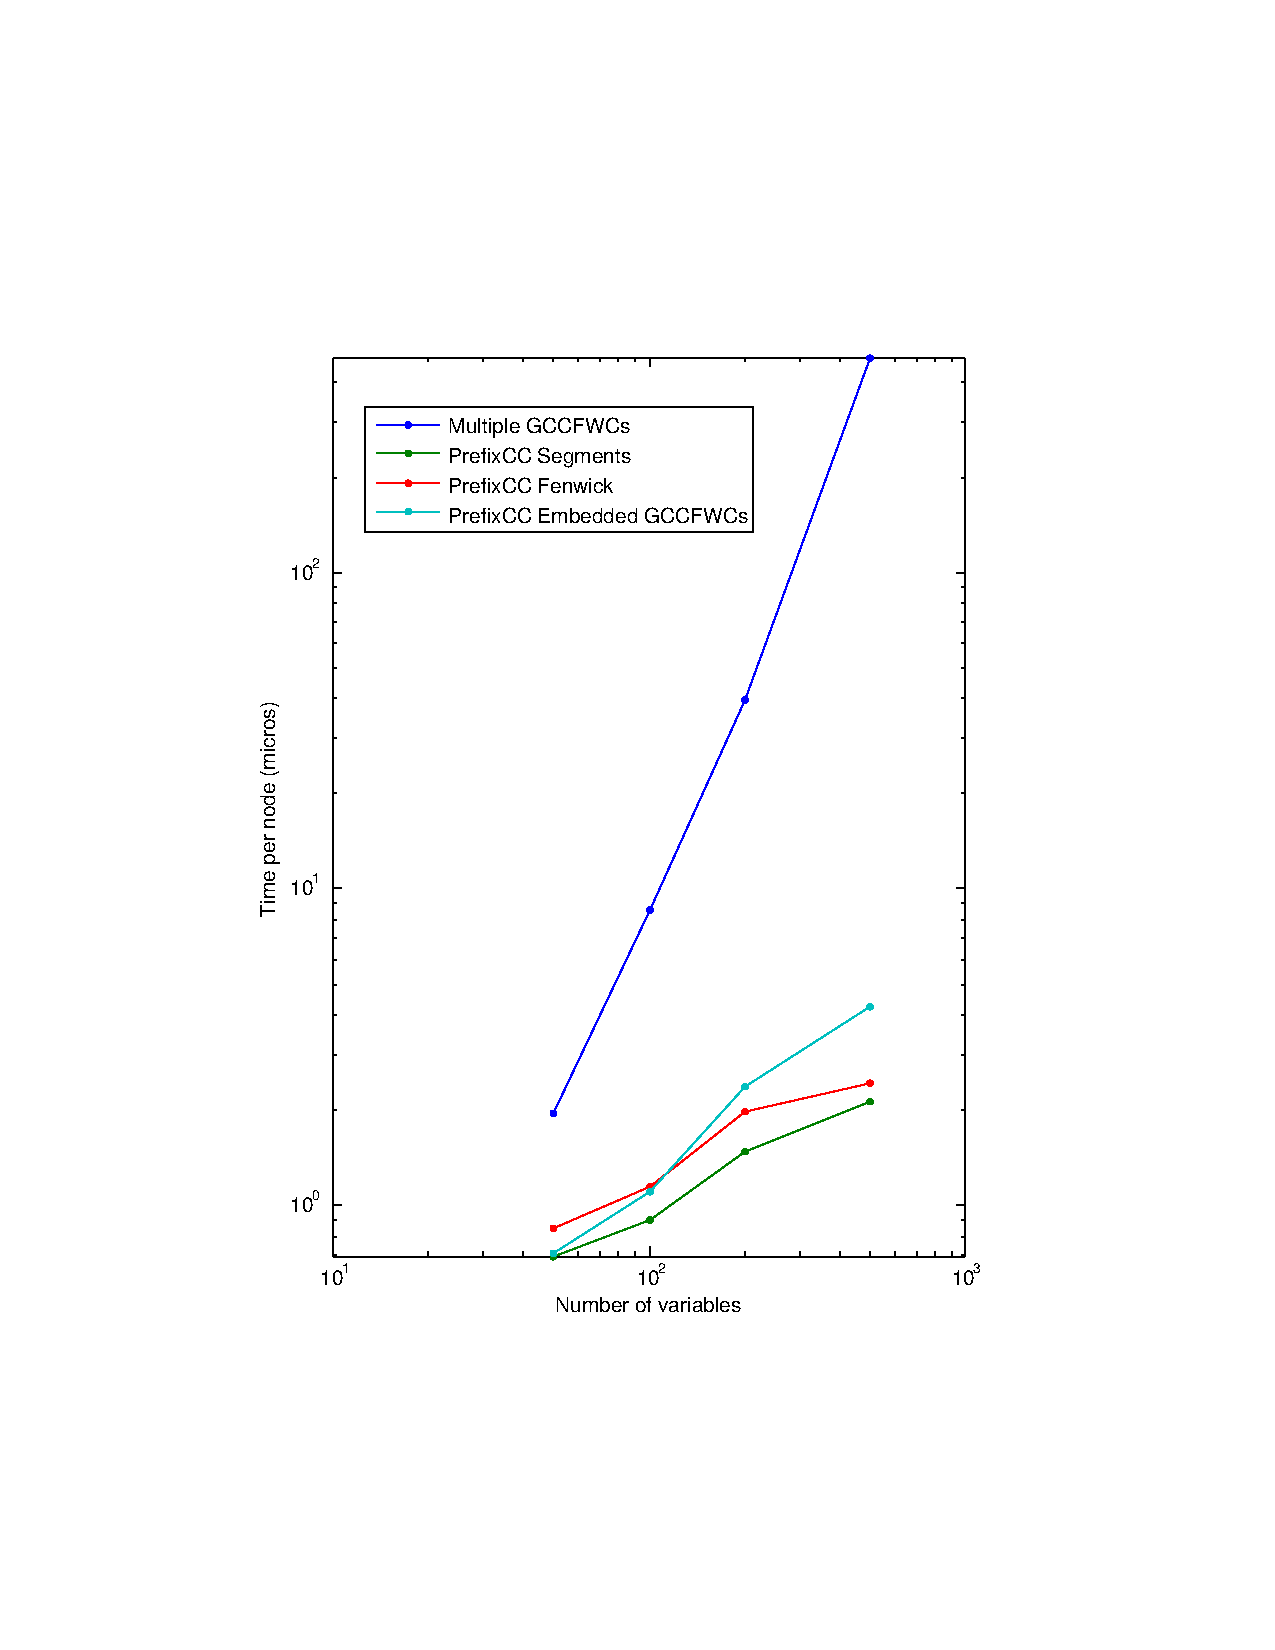
\includegraphics[trim = 4cm 6cm 4cm 6cm, width=0.5\textwidth]{img/loglog-graph}
    \caption{The time spent on a node can increase greatly with the number of variables.}
    \label{fig:loglog-complexity}
\end{figure}

We can see that as predicted the approaches that use regular GCCFWCs suffer greatly from the increase because of their redundancy, especially \emph{Multiple GCCFWCs} which uses a separate constraint for each prefix. The time for the other two approaches grows much more reasonably and thus they are better fit for larger instances.

With that first intuition, we then performed more tests at 50, 100 and 200 variables and made performance profiles with the \emph{Multiple GCCFWCs} approach as a baseline. Figure~\ref{fig:weak-all-time-static} shows the summarized time profile for those three batches.

\begin{figure}
    \centering
    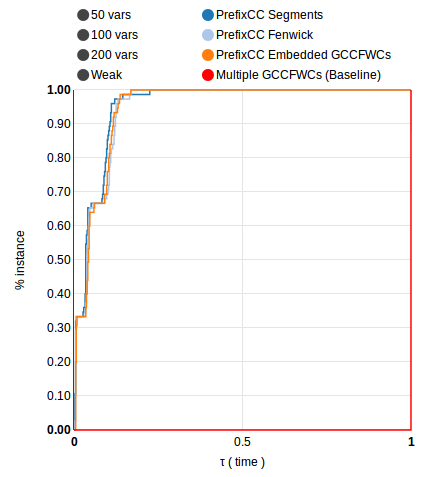
\includegraphics[width=0.5\textwidth]{img/weak-all-time-static}
    \caption{The \emph{Multiple GCCFWCs} approach is clearly distanced in running time by the new approaches.}
    \label{fig:weak-all-time-static}
\end{figure}

We can see that all three new approaches are much faster than the \emph{Multiple GCCFWCs} approach, which confirms the results we saw in figure~\ref{fig:loglog-complexity}. In addition, we can see three blocks in the time ratios, corresponding from top to bottom to the 50-variables, the 100-variables and the 200-variables batches of tests. They are due to the strong sensibility of our baseline to the number of variables, which also we saw in the previous graph.

As this view does not give much information in the difference between the three other approaches, we also made a profile of the running times relative to the best approach for the each test case, which is shown in figure~\ref{fig:weak-all-time}.

\begin{figure}
    \centering
    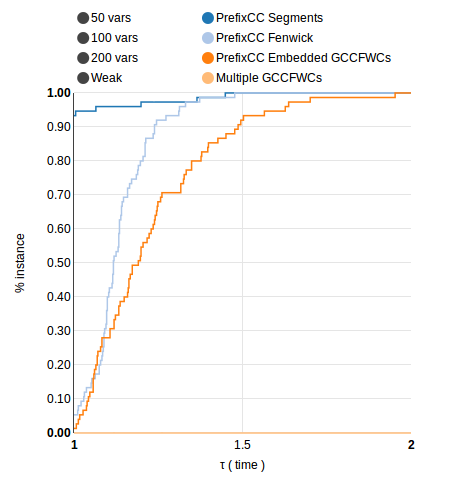
\includegraphics[width=0.5\textwidth]{img/weak-all-time}
    \caption{The \emph{PrefixCC Segments} approach is fastest for a wide majority of the test cases.}
    \label{fig:weak-all-time}
\end{figure}

We can see here that the curve for the \emph{PrefixCC Segments} approach only leaves the value 1 above the $0.9$ mark in the instance share, which means it is the fastest approach for more than 90\% of the instances. We also see that the \emph{PrefixCC Fenwick} approach seems to be faster in most cases than the \emph{PrefixCC Embedded GCCFWCs} approach, but we will have to take a closer look. Finally, we note that the \emph{Multiple GCCFWCs} approach is, predictably, out of the graph.

To get a better idea of the relative performance of the these approaches, we have to look at the three test batches separately. Figure~\ref{fig:weak-separate} shows us the performance profiles for 50, 100 and 200 variables.

\begin{figure}
    \centering
    \begin{subfigure}[b]{0.3\textwidth}
        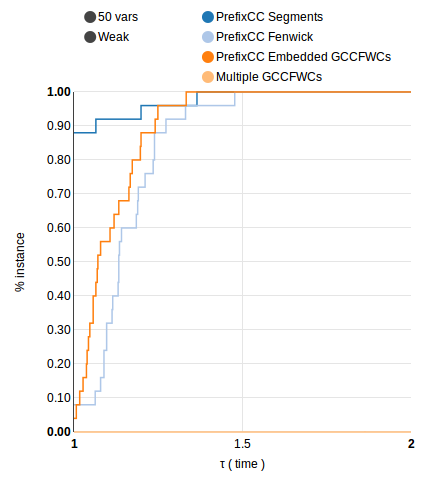
\includegraphics[width=\textwidth]{img/weak-50vars-time}
        \caption{Time at 50 variables}
    \end{subfigure}
    \quad
    \begin{subfigure}[b]{0.3\textwidth}
        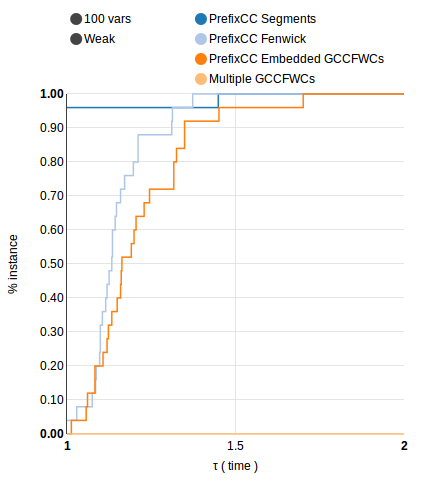
\includegraphics[width=\textwidth]{img/weak-100vars-time}
        \caption{Time at 100 variables}
    \end{subfigure}
    \quad
    \begin{subfigure}[b]{0.3\textwidth}
        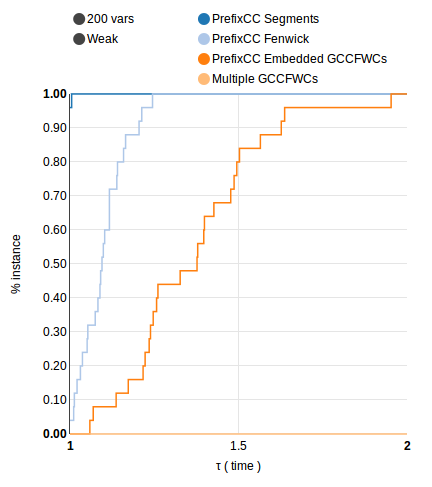
\includegraphics[width=\textwidth]{img/weak-200vars-time}
        \caption{Time at 200 variables}
    \end{subfigure}
    
    \caption{As the number of variables increases, \emph{PrefixCC Embedded GCCFWCs} has more and more difficulty keeping up with the speed of the other two approaches.}
    \label{fig:weak-separate}
\end{figure}

By looking at the evolution of the relative running time in those three cases, we can see that while \emph{PrefixCC Fenwick} stays quite stable with relation to \emph{PrefixCC Segments}, the \emph{PrefixCC Embedded GCCFWCs} approach has its performance worsen with every factor two. Again, this confirms the results we expected from figure~\ref{fig:loglog-complexity}.

To summarize the results of these weak constraints tests, we can say that \emph{Multiple GCCFWCs} and to a lesser extent \emph{PrefixCC Embedded GCCFWCs} have running times that increase too quickly with the number of variables (or equivalently, the number of bounds) while the other two approaches show similar and more reliable performances.

\subsection{Harder tests}
\label{subsec:results-hard}

We will now look at the results of the harder tests we performed, whose aim was to give an advantage to the solutions with the better pruning. We will look in particular at the \emph{PrefixCC Fenwick} approach, which has the strongest pruning of the four.

Let us begin by looking at the relative time, first with our usual baseline \emph{Multiple GCCFWCs} and then at the time relative to the fastest approach. They are both shown in figure~\ref{fig:hard-time}.

\begin{figure}
    \centering
    \begin{subfigure}[b]{0.45\textwidth}
        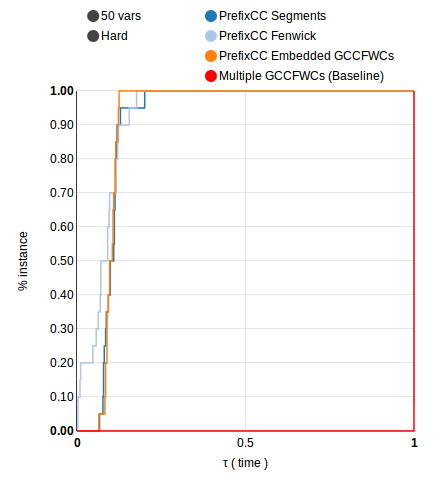
\includegraphics[width=\textwidth]{img/hard25-50vars-time-static}
        \caption{Time relative to the baseline}
        \label{fig:hard-time-static}
    \end{subfigure}
    \quad
    \begin{subfigure}[b]{0.45\textwidth}
        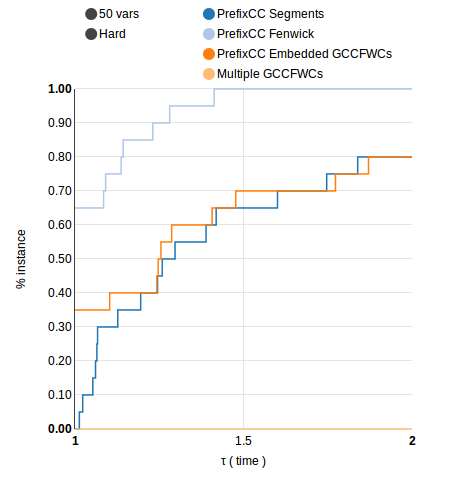
\includegraphics[width=\textwidth]{img/hard25-50vars-time}
        \caption{Time relative to the fastest approach}
        \label{fig:hard-time-dynamic}
    \end{subfigure}
    
    \caption{The \emph{PrefixCC Fenwick} approach acquires a strong advantage in running time for most of the test cases.}
    \label{fig:hard-time}
\end{figure}

We can first see in figure~\ref{fig:hard-time-static} that most approaches keep a profile quite similar to the weakly constrained tests while the \emph{PrefixCC Fenwick} approach manages to take much less time than other approaches on some test cases. On the right in figure~\ref{fig:hard-time-dynamic}, we observe that this approach has become the fastest approach for 65\% of the tests.

Since the \emph{PrefixCC Fenwick} approach is supposedly slower per node than the \emph{PrefixCC Segments} approach (see previous subsection), this can only mean that it has performed more pruning, which we check in figure~\ref{fig:hard-backtracks}.

\begin{figure}
    \centering
    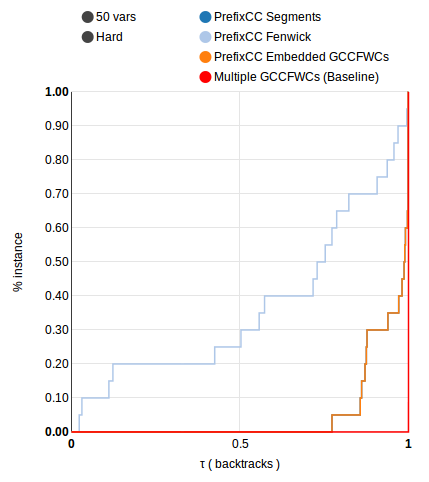
\includegraphics[width=0.5\textwidth]{img/hard25-50vars-backtracks}
    \caption{The \emph{PrefixCC Fenwick} approach has in most cases a much better pruning than the other three approaches.}
    \label{fig:hard-backtracks}
\end{figure}

We see that \emph{PrefixCC Segments} and \emph{PrefixCC Embedded GCCFWCs} (which overlap in the graph) have performed some additional pruning relative to the baseline, but by far the most significant pruning is made by the \emph{PrefixCC Fenwick} approach, which for 30\% of the cases had only half as many backtracks as the baseline. This accounts for its improved running time.

In addition, we mentioned in the test description (see \ref{subsec:tests-hard}) that in order to get accurate performance profiles we had to limit the difficulty of the test cases, since for tests with stronger bounds that the \emph{PrefixCC Fenwick} approach solved easily, the other three solutions timed out before finding any solution.

To summarize the results of these harder tests, we can say that for cases where pruning is important, the \emph{PrefixCC Fenwick} approach gains a strong advantage in running time despite being less efficient per node than the \emph{PrefixCC Segments} approach.

\section{Conclusion}

We saw in subsection~\ref{subsec:results-weak} that the \emph{PrefixCC Segments} approach was the most efficient regardless of numbers of variables for tests where strong pruning was not critical to search speed. We also saw in subsection~\ref{subsec:results-hard} that the \emph{PrefixCC Fenwick} approach had a strong pruning that helped greatly for problems with relatively tight bounds and made it overall faster than the \emph{PrefixCC Segments} approach.

Therefore, we recommend using the \emph{PrefixCC Segments} approach by default in situations with relatively weak bounds and with other fast constraints because of its propagation speed, while the \emph{PrefixCC Fenwick} approach should be the preferred option when pruning becomes important and eliminating nodes could lead to faster searches despite its slower speed per node.

\end{document}
